\chapter{Classification schemes}
In this chapter a few classification models are evaluated for the feature extraction processes described in the preceding chapter. Detailed descriptions of each classification framework is omitted, but good sources for further explanation will be supplied for the interested reader. The aim of this chapter is to compare various models and to determine the most promising one with regards to accuracy, size and complexity. 

\section{Linear Models}
Linear models are widely used in practice as they are general, and can therefore be used in many cases \citep{shalev-shwartz_ben-david_2016}.  Furthermore, they are relatively easy to understand, in contrast to more complex models such as neural networks. Despite this, they can often produce a decent accuracy with a low complexity.

In this work, two linear models are considered. One being \emph{Linear Discriminant Analysis} (LDA) and the other, \emph{Support Vector Machine} (SVM) with a linear kernel. 

\subsection*{Linear Discriminant Analysis}
Linear Discriminant Analysis, or LDA for short, is an algorithm commonly used for dimensionality reduction of data. \citep{raschka_2014} It is not uncommon, however, to use it for classification tasks as well. LDA is a supervised algorithm, meaning it knows what class each sample belongs to. This enables it to project data into a lower dimension in such a way that the different classes are as separated as possible; unlike PCA which projects data in a way that maintains a high variance, disregarding class labels. 

Reducing the dimensionality of data is a good way of both lowering computational costs and avoiding overfitting as well as other phenomena that stem from a high-dimensional data.

For further reading about LDA, we refer to \citep{raschka_2014}.

\subsection*{Support Vector Machine}
SVMs are one of the most popular models when it comes to supervised learning. The most simple SVM uses what is called a linear kernel, and generates a linear hyperplane that separates two sets of labeled data. Finding such a hyperplane is often an ambiguous task, so to find what the SVM regards as the best hyperplane, it seeks parameters that maximize the distance between the hyperplane and the sample points closest to it, known as support vectors \citep{boswell2002introduction}.

Even if support vector machines are linear models, they are not limited to work only on linearly separable data. There are ways to use them in a non-linear fashion by utilizing different kinds of kernels \citep{xia_2016}. In principle, the data is first transformed into a higher dimensional space, including non-linear terms. In this new space, the SVM is used just as before. This makes the SVM a powerful tool even in non-linear problems.

\section{Non-linear Models}

\subsection*{Random Forest}
Random Forest (RF) is a strong tool that can be used for both regression- and classification problems. The name stems from that the method is based on several \textit{decision trees}, which are initiated randomly. A decision tree is a classifier per se, and is structured as a sequence of simple questions. These questions typically ask if a sample's feature is equal to, or greater/smaller than some set value. The answers to these questions form a path in the decision tree, leading to an end node which corresponds to the prediction.

RF segments the training data into $n$ parts, and induces a decision tree from each group of data. Thus there are $n$ predictors that work independently, and by selecting the most common prediction, RF yields a robust result with no overfitting due to the combined results of many trees. On top of that it offers a very high accuracy in a wide variety of applications, while still maintaining an intuitive model structure that allows us to, e.g., estimate which features are important. \citep{breiman_cutler_2018}


\subsection*{Logistic Regression}
Logistic regression is simlar to an ordinary linear regression. Both methods aim to estimate parameters to describe the relationship between the input- and the output variables. For linear regression, the parameters $\{b_i\}_{i=0}^n$ are estimated, and together with the input variables $\{X_i\}_{i=1}^n$ they generate the output $Y$:

\begin{equation}
	Y= b_0+\sum_{i=1}^n b_iX_i.
\end{equation}

One big difference between the two models is that linear regression outputs continuous values, whereas logistic regression outputs a value in the open interval (0,1).  To achieve this, logistic regression transforms the result of the linear regression using the sigmoid function, defined as $f(z)=\frac{1}{1+e^{-z}}$. With this function, logistic regressions maps the inputs $X_i, i=1,...,n$ to
\begin{equation}
	Y= \frac{1}{1+e^{-b_0-\sum_{i=1}^n b_iX_i}}
\end{equation}

This value is interpreted as a probability and can be used for making a decision in a binary classification - in this case grass/not grass.

Another major difference between linear and logistic regression is the choice of cost function. Logistic regression commonly uses a cost function known as Cross-Entropy or Log Loss as opposed to Mean Squared Error, which is used for linear regression. For further details about logistic regression, including its cost function, we refer to \citep{a_smola_svn_vishwanathan_2010}.

\subsection*{Artificial neural networks}

Artificial neural networks (ANNs) constitute a class of nonlinear models designed to mimic biological neural systems. ANNs consist of multiple layers of neurons. 


ANNs have been widely applied to solve a great number of difficult problems in different areas, including pattern recognition, signal processing and language learning. 


\subsection*{LSTM}
In previous models the data went through a feature extraction process before going into the model training. For this model, on the other hand, no feature extraction is performed. Instead, several consecutive sweeps of unprocessed IQ-data are used as input. Each range bin can be regarded as a one-dimensional time series. This motivates the use of some classification scheme that exploits temporal behaviour. Recurrent neral networks (RNNs) feature this by having feedback within individual layers in the network. \citep{karim_majumdar_darabi_chen_2018} The problem with RNNs, however, is that they suffer from a vanishing or exploding gradient, and can only sustain a short term memory. A way to combat this is to use a neural network layer called long short term memory (LSTM).

LSTM-layers have previously been used successfully for classifications in radar applications. For instance in \citep{jithesh_sagayaraj_srinivasa_2018} the method was able to classify flying objects from $\textbf{nnn}$ different classes with an accuracy of ...? The theory behind these layers are thoroughly described in, for example \citep{hochreiter_schmidhuber_1997}

Mention some source(s) using convolutional layers for radar classification.

 In \citep{karim_majumdar_darabi_chen_2018}, the LSTM layer is used in combination with a fully convolutional neural network (FCN), which proves to be a significant improvement from just using FCNs when classifying time series.

Describe our model.

\subsection*{Feedforward neural networks}
Feedforward networks consist of an input layer, some hidden layers and an output layer. Each layer receives a set of input values $\mathbf{x}$ from the previous layer, multiplies the inputs by a set of weights $\mathbf{\beta}_{i}$ and applies a nonlinear activation function $F$ to the multiplication output. This output is then used as inputs for the sequent layer. The output of layer $i$ at neuron index $j$, $y_{i,j}$, is thus related to the previous layer output $\{{y}_{i-1, k}\}_{k=1}^{K}$ through

\begin{equation}
	y_{i,j} = F\Big\{\sum_{k=1}^{K}\beta_{i,j,k}y_{i-1,k}\Big\}
\end{equation}




Deep neural networks, or DNN for short, are neural networks that has more than one layer of hidden units between its inputs and outputs \citep{hinton_deng_yu_dahl_mohamed_jaitly_senior_vanhoucke_nguyen_sainath_2012}. 


DNN's in various forms have gained immense popularity over the past two decades achieving considerable success within a wide spectrum of applications, such as in image recognition \citep{szegedy_liu_jia_sermanet_reed_anguelov_erhan_vanhoucke_rabinovich_2018}, acoustic modeling of speech \citep{hinton_deng_yu_dahl_mohamed_jaitly_senior_vanhoucke_nguyen_sainath_2012}, 



% Define block styles
\tikzstyle{decision} = [diamond, draw, fill=blue!20, 
    text width=7.5em, text badly centered, inner sep=0pt]
\tikzstyle{block} = [rectangle, draw, fill=blue!20, 
    text width=7em, text centered, rounded corners, minimum height=4em]
\tikzstyle{line} = [draw, -latex']
\tikzstyle{cloud} = [draw, ellipse,fill=red!20, node distance=3cm,
    minimum height=4em]
\tikzstyle{blockgreen} = [rectangle, draw, fill=green!20, 
    text width=7em, text centered, rounded corners, minimum height=4em]
\tikzstyle{blockbrown} = [rectangle, draw, fill=brown!20, 
    text width=7em, text centered, rounded corners, minimum height=4em]

\begin{figure}
\centering
\begin{tikzpicture}[node distance = 3cm, auto]
	% Place nodes
	\node [blockbrown] (obtained) {Obtained data};
	\node [blockgreen, below left of=obtained] (training) {Training data};
	\node [block, below right of=obtained] (test) {Test data};
	\node [blockgreen, below of=training, node distance=2.2cm] (train pre) {Preprocess and extract features};
	\node [block, below of=test, node distance=2.2cm] (test pre) {Preprocess and extract features};
	\node [blockgreen, below right of=train pre] (est) {Estimate $\mathbf{\mu}_f$, $\mathbf{\sigma}_f$};
	\node [blockgreen, below left of=est] (scale train) {Scale to ZMUV};
	\node [block, below right of=est] (scale test) {Scale to ZMUV};
	\node [cloud, below right of=scale train] (train model) {Train model};
	\node [decision, below of=train model] (classify) {Classification};
	\node [block, below of=classify] (post) {Postprocessing};
	\node [block, below of=post, node distance=2.2cm] (output) {Model output};
	% Draw lines
	\path [line] (obtained) -| (training);
	\path [line] (obtained) -| (test);
	\path [line] (training) -- (train pre);
	\path [line] (test) -- (test pre);
	\path [line, dashed] (train pre) -| (est);
	\path [line,dashed] (est) -- (scale train);
	\path [line,dashed] (est) -- (scale test);
	\path [line] (test pre) -- (scale test);
	\path [line] (train pre) -- (scale train);
	\path [line] (scale train) |- (train model);
	\path [line] (train model) -- (classify);
	\path [line] (scale test) |- (classify);
	\path [line] (classify) -- (post);
	\path [line] (post) -- (output);
\end{tikzpicture}
\caption{Flowchart of classification scheme.}
\end{figure}



\rowcolors{2}{gray!25}{white}
\begin{table}
	\begin{center}
	\begin{adjustbox}{totalheight=\textheight-2\baselineskip}
		\begin{tabular}{|l|l|l|l|l|l|l|}
		\hline
		\rowcolor{gray!150}
		\rule{0pt}{25pt}\color{white}\textbf{Material} & \color{white}\textbf{LR} & \color{white}\textbf{RF} & \color{white}\textbf{\shortstack{LSTM\\CNN}} & \color{white}\textbf{SVM} & \color{white}\textbf{LDA} & \color{white}\textbf{DNN}\\
		pgrass1 & 97.9 & 98.05 & \cellcolor{red!20}59.0 & 95.75 & 96.8 & 97.45\\
		pgrass3 & 99.8 & 99.5 & \cellcolor{red!20}83.8 & 96.2 & 100.0 & 99.95\\
		pgrass4 & 94.35 & \cellcolor{red!20}86.75 & 94.5 & 91.4 & 92.6 & 95.3\\
		pgrass5 & 95.7 & 96.45 & 100.0 & 91.35 & 93.65 & 97.8\\
		qgrass1 & 96.65 & 97.25 & 97.4 & 93.95 & 95.9 & 95.55\\
		qgrass2 & 96.35 & 98.8 & 95.9 & 92.95 & 97.2 & 99.3\\
		qgrass3 & 99.9 & 99.85 & 99.9 & 99.65 & 99.95 & 100.0\\
		hgrass12 & 97.0 & 96.65 & 97.5 & 96.85 & 92.7 & 96.95\\
		hgrass2 & 97.75 & 97.7 & 99.8 & 97.8 & 96.3 & 98.75\\
		hgrass3 & 99.2 & 98.65 & 99.9 & 99.0 & 97.65 & 99.7\\
		hgrass4 & 99.35 & 98.7 & 99.9 & 99.25 & 97.55 & 99.8\\
		hgrass5 & 99.6 & 99.4 & 99.9 & 99.6 & 99.2 & 99.65\\
		hgrass6 & 100.0 & 100.0 & 100.0 & 100.0 & 99.85 & 100.0\\
		hgrass7 & 96.35 & 96.8 & 98.6 & 95.6 & \cellcolor{red!20}89.85 & 98.1\\
		hgrass8 & 97.6 & 95.45 & 99.8 & 93.1 & \cellcolor{red!20}87.4 & 99.05\\
		hgrass9 & 97.55 & 98.0 & 99.8 & 95.8 & 94.05 & 98.85\\
		hgrass10 & 95.4 & 92.85 & 98.4 & 94.6 & \cellcolor{red!20}89.9 & 95.0\\
		hgrass11 & 97.35 & 94.4 & 96.9 & 96.55 & 93.65 & 95.6\\
		pasph1 & 100.0 & 100.0 & 99.9 & 100.0 & 100.0 & 100.0\\
		pgravel1 & 99.45 & 99.85 & 99.8 & 99.9 & 99.2 & 99.7\\
		pasph2 & 99.95 & 100.0 & 99.0 & 100.0 & 100.0 & 100.0\\
		pasph3 & 100.0 & 100.0 & 99.7 & 100.0 & 99.95 & 99.2\\
		psoil1 & 99.85 & 100.0 & 99.7 & 99.95 & 99.7 & 99.9\\
		psoil2 & 99.35 & 99.6 & 99.4 & 99.85 & 99.4 & 99.75\\
		ptiles1 & 99.35 & 99.4 & 100.0 & 99.55 & 99.3 & 99.35\\
		qasph1 & 99.9 & 99.85 & 100.0 & 99.9 & 99.95 & 100.0\\
		qasph2 & 100.0 & 100.0 & 100.0 & 100.0 & 100.0 & 100.0\\
		qgravel1 & \cellcolor{red!20}82.65 & 97.1 & \cellcolor{red!20}86.6 & \cellcolor{red!20}88.2 & \cellcolor{red!20}89.3 & 94.3\\
		qsoil1 & 99.75 & 99.85 & 100.0 & 100.0 & 99.9 & 99.85\\
		qsoil2 & 97.8 & 96.3 & \cellcolor{red!20}88.9 & 98.9 & 97.4 & 95.95\\
		qtiles1 & 99.95 & 99.75 & 99.9 & 99.95 & 99.6 & 99.95\\
		rtiles1 & 99.95 & 99.9 & 100.0 & 100.0 & 100.0 & 99.95\\
		rgravel1 & 99.95 & 99.55 & 100.0 & 100.0 & 99.95 & 99.75\\
		rgravel2 & 98.95 & 99.6 & 99.9 & 99.55 & 99.9 & 99.8\\
		rasp1 & 100.0 & 100.0 & 100.0 & 100.0 & 99.9 & 99.95\\
		rsoil1 & 96.25 & 95.45 & 100.0 & 96.55 & 96.55 & 93.95\\
		G2gravel2 & 99.85 & 99.8 & 99.9 & 99.95 & 100.0 & 99.7\\
		G2gravel1 & 99.75 & 99.7 & 100.0 & 99.75 & 99.9 & 99.55\\
		G2soil1 & 96.35 & 94.0 & 99.3 & 96.85 & 95.5 & 99.85\\
		G2tiles1 & 99.95 & 99.7 & 99.5 & 99.95 & 100.0 & 94.45\\
		hsoil1 & 92.65 & 95.15 & 99.3 & 90.25 & 92.4 & 100.0\\
		hsoil2 & 94.75 & 95.65 & \cellcolor{red!20}84.7 & 90.95 & 92.9 & 95.15\\
		\hline
		\textbf{Mean} & 97.96 & 97.99 & 97.06 & 97.37 & 97.02 & \cellcolor{green!20}98.5\\
		\textbf{Median} & 99.35 & 99.4 & \cellcolor{green!20}99.8 & 99.4 & 99.2 & 99.68\\
		\textbf{SD} & 3.05 & 2.63 & 7.23 & 3.3 & 3.58 & \cellcolor{green!20}1.96\\
		\hline
		\end{tabular}
	\end{adjustbox}
	\end{center}
	\label{tab:loo}
	\caption{Leave-one-out accuracies for all collected data series and several different models.}
\end{table}


\section{Model evaluations}
Model evaluation is an important aspect in creating machine learning models. By using a bad evaluation strategy, one might construct a model that is seemingly good, but turns out to be useless in reality, simply because the model has been evaluated using a poorly chosen set of data. There are several things to keep in mind when testing a model's performance. One of these is to use evaluation metrics that are relevant to the type of model that is being tested. For a classification model, a common metric is accuracy, which reveals the ratio between correct predictions and total predictions. A more informative metric is the confusion matrix which, in addition, provides details about the model's mispredictions. Two additional metrics, suitable for classification are log-loss and AUC \citep{zheng_2015}. 

However, selecting a suitable metric is not enough. Of course, choosing what data to test your model on is equally important. By predicting on data that the model has been trained on, one could expect a very high accuracy. This accuracy, however, is not interesting at this point as a model is intended to be used on new, unseen data. For this reason, the dataset is split up in a training set and a test set in one of many ways \citep{raschka}.


\subsubsection{Validation Set Accuracy}
Splitting a dataset into a training and validation set often means selecting samples for training and validation completely randomly. This can be a good way of comparing different models' performances, but it is not the ideal method for a final model evaluation. While it is true that the validation set consists of samples that the model has never seen before, it \textit{has} trained on samples close to the validation samples due to the random selection. Oftentimes closely spaced samples can have a high resemblance, and even if the model has not trained on the validation samples, it achieves a high validation accuracy because it has trained on very similar samples.

\begin{figure}[h]
	\centering
	
\includegraphics[scale=0.3]{figs_temp/validation_split.jpg}
	\caption{Splitting a dataset into a training- and validation set usually refers to selecting a certain percentage of samples at random and evaluate the model based on those.}
	\label{fig:validation_split}
\end{figure}

\subsubsection{Leave-one-out accuracy}
The leave-one-out strategy means dividing the dataset into $n$ parts. The model validation is then performed in $n$ stages. For each stage, the model is trained on all data, except for one of the $n$ parts, as in figure \ref{fig:loo}. After the training, the model makes predictions of the unseen data, and the accuracy is noted. When having a small dataset - or as in this case, an arguably small amount of surfaces that have been recorded - this method is useful in that it does not require us to withhold data from the model training \citep{raschka}. It also mimics a real scenario where the model predicts on a surface it has never seen before.

In table \ref{tab:loo}, the leave-one-out results of all models above are listed for comparison.

\begin{figure}[h]
	\centering
	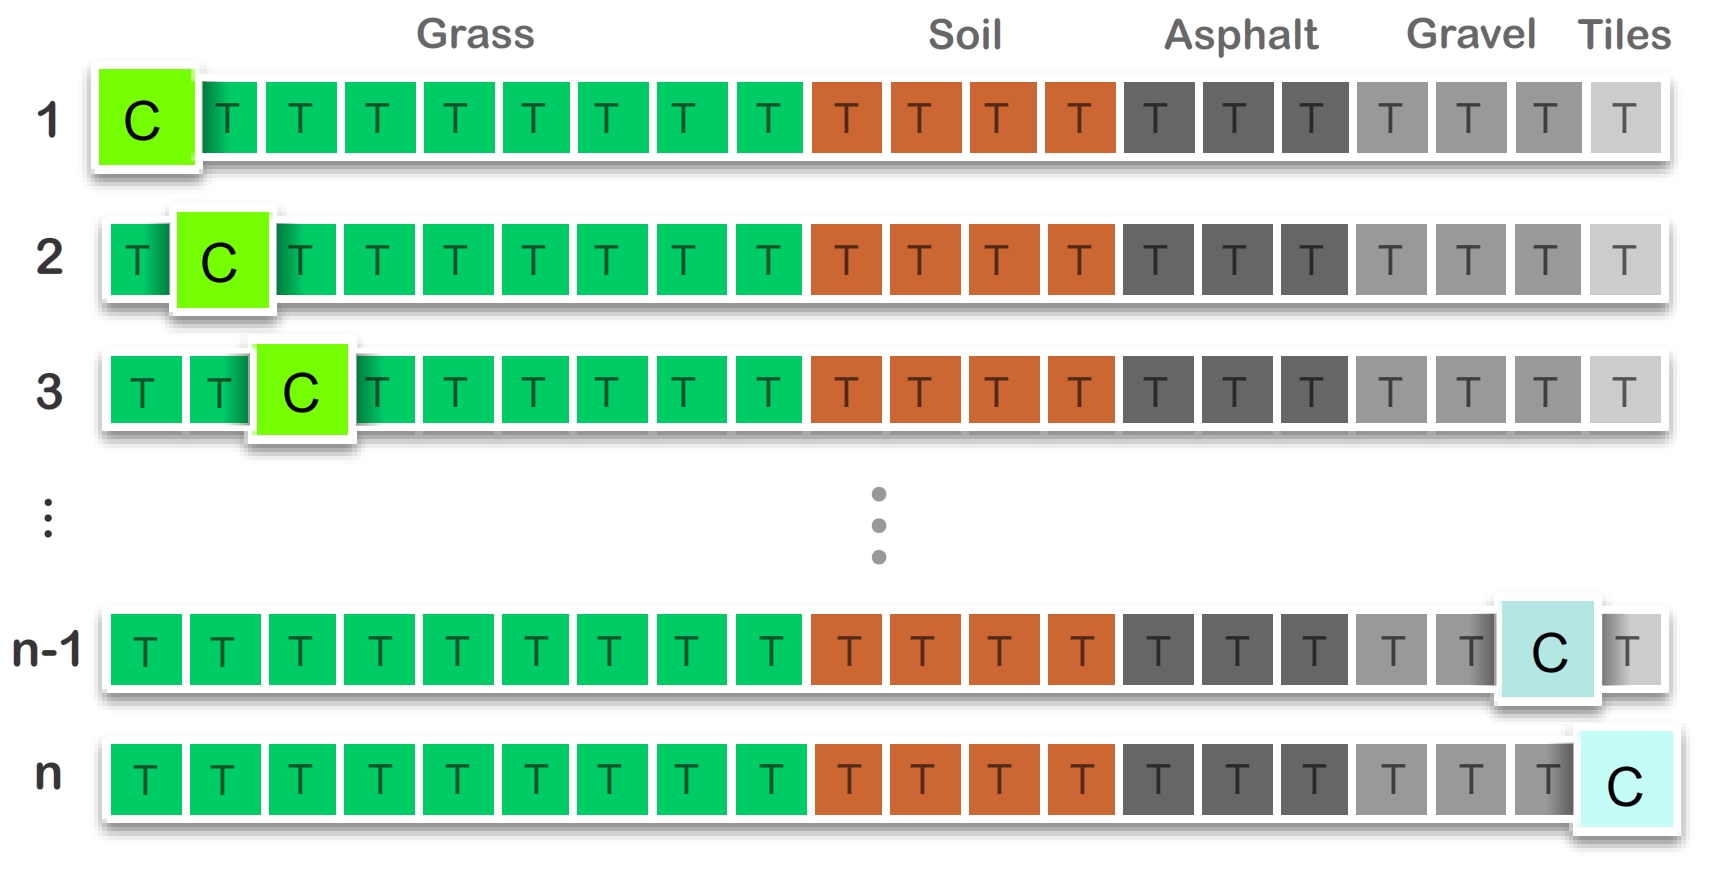
\includegraphics[scale=0.3]{figs_temp/loo.jpg}
	\caption{With the leave-one-out strategy, data is split up into $n$ parts. The model evaluation is done in $n$ steps - each time, one part of the data is excluded from the training and evaluated upon. The T's in the figure mark which parts of the data that are used for training, and the C's show what is used for classification.}
	\label{fig:loo}
\end{figure}

\subsubsection{Selecting a Model}
Optimizing each model presented above would of course be ideal, but also require much time and effort. Hence, we select what we regard as the most promising model based on the aforementioned evaluation methods. This model will then be optimized and more thoroughly evaluated.

In table ... we see the validation accuracies of all models. <Some comment about the result...> bla bla bla

Table \ref{tab:loo} shows the leave-one-out results for all models. These are more interesting as the model is evaluated on surfaces it has never before seen. From the table we can see that all models perform well on every asphalt- and tiled surfaces. Gravel-, soil- and grass-surfaces, however, can sometimes be harder to classify for the models. Looking back at the principal component analysis in figure *ref to PCA-plot*, this is what we could have expected due to the wide spread, and slight overlap between the samples within these categories. As for gravel, there is one measurement in particular that sticks out - "qgravel1". The accuracy of this is well below the average accuracy for all models. This could be that this particular gravel contains characteristics which are not captured by the other non-grass surfaces, resulting in several misclassifications. It could also be that some temporary problem occured while measuring, for example that the radar jumped out of its socket.

Another quirk worth noting is the great accuracy span of the LSTM\& CNN method. While it has a leading median score of 99.8 \%, it also contains several dips to some of the lowest accuracies of all models. This gives it a high standard deviation compared to the other models, and makes it less robust. It is possible that this could be remedied with a little bit of fine-tuning, but due to a limited amount of time, we disregard the LSTM-model, and the DNN-model becomes the one with the greatest median and mean as well as the lowest standard deviation.








